% !TEX root = ../thesis-sample.tex

\chapter{Setting}
The next chapter has the good stuff.

\section{Convergence Criteria}
Actually, it might have the worst stuff.  But it is slightly easier to
write than the material in Chapter \ref{chap:intro}.

\begin{figure}
 \begin{center}
  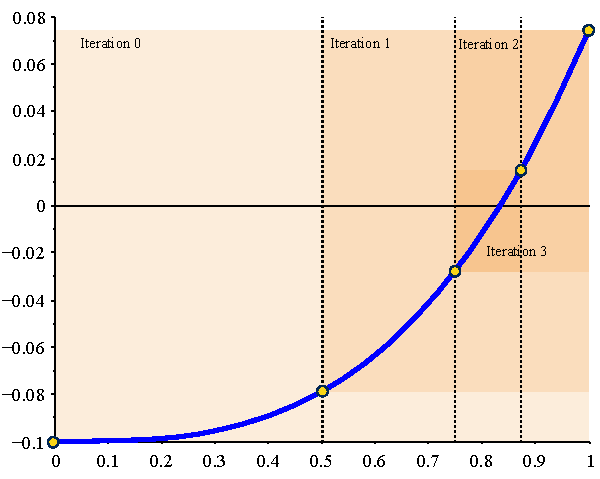
\includegraphics[scale=1]{./figures/f1_tol.pdf}
 \end{center}
 \caption{ \label{fig:fn:tol}
  Illustration of $x$- and $y$-tolerances for bisection iterations}
\end{figure}

\newpage

It takes very little text to fill a page in this format, but there is even less text on most of these sample pages.

\section{Why we are doing it}
It is usually a good idea to give reasons for your research.  If you do not, the people who paid you to waste all that time will feel really bad about it, and then they will not provide the same opportunity to future students.

\newpage

I need this page to see what even-numbered pages look like.